\documentclass[final,MD,numbers,times,AutoFakeBold]{cumtthesis}
% 参数1:文档格式  预印版\终稿\盲审\检查 preprint, final, blindreview, check
%       写作可用preprint, 打印时修改为 final, 仅考虑本科生模板,暂时不支持盲审\检查格式
% 参数2:学位  本科\硕士\博士 BD MD PhD
%       仅考虑本科生模板,暂时不支持硕士\博士格式,这里有bug未解决,本科生还是选择MD即可
\usepackage{fontspec}
\usepackage{textcomp, gensymb}
\setmainfont{Times New Roman}
\usepackage{listings}
\usepackage{multirow}
\usepackage{indentfirst}
\usepackage{tikz}
\usepackage{etoolbox}
\usepackage{color}
% 使用更新的伪代码包写法
\usepackage{algorithm}
\usepackage{algpseudocodex}
\usepackage{float}
\usepackage{rotating}
\usepackage{booktabs}
\usepackage{enumerate}
\usepackage{emptypage}
\usepackage[a4paper,left=3.17cm,right=3.17cm,top=2.54cm,bottom=2.54cm]{geometry}
\usetikzlibrary{matrix,calc,shapes,backgrounds,patterns,positioning,decorations.pathreplacing}
%=================================== 数学符号 =================================%
\newcommand{\rtn}{\mathrm{\mathbf{R}}}
\newcommand{\N}{\mathrm{\mathbf{N}}}
\newcommand{\AS}{~\mathrm{a.s.}}
\newcommand*{\PR}{\mathrm{\mathbf{P}}}
\newcommand*{\EX}{\mathrm{\mathbf{E}}}
\newcommand*{\dif}{\,\mathrm{d}}
\newcommand*{\F}{\mathcal{F}}
\newcommand*{\prs}{\dif\PR-\mathrm{a.s.}}
\newcommand*{\pts}{\dif\PR\times\dif t-\mathrm{a.e.}}
\newcommand{\Ito}{It\^{o}}
\newcommand{\tT}[1][0]{[#1,T]}
\newcommand{\intT}[2][T]{\int^{#1}_{#2}}
\newcommand{\s}{\mathcal{S}}
\newcommand{\me}{\mathrm{e}}
\newcommand{\one}[1]{{\bf 1}_{#1}}
\newcommand{\Mm}{{\rm M}}
\newcommand{\circled}[2][]{\tikz[baseline=(char.base)]
    {\node[shape = circle, draw, inner sep = 1pt]
    (char) {\phantom{\ifblank{#1}{#2}{#1}}};%
    \node at (char.center) {\makebox[0pt][c]{#2}};}}
\robustify{\circled}
\setlength{\intextsep}{10.0pt plus 2.0pt minus 2.0pt}

\DeclareMathOperator*{\sgn}{sgn}
%=================================== 数学符号 =================================%
%=================================== Code Style ==============================%
\definecolor{mygreen}{rgb}{0,0.6,0}
\definecolor{mygray}{rgb}{0.5,0.5,0.5}
\definecolor{mymauve}{rgb}{0.58,0,0.82}
\lstset{
    aboveskip=3mm,
    belowskip=3mm,
    showstringspaces=false,
    columns=flexible,
    basicstyle={\normalsize\ttfamily},
    numbers=left,
    frame=L,
    numberstyle=\tiny\color{mygray},
    keywordstyle=\color{blue},
    commentstyle=\color{mygreen},
    stringstyle=\color{mymauve},
    breaklines=true,
    breakatwhitespace=true,
    tabsize=3,
    framextopmargin=2pt,framexbottommargin=2pt,abovecaptionskip=-3pt,belowcaptionskip=3pt,    
    xleftmargin=1em, % 设定listing左右的空白
}

\begin{document}
% 正文前部分
\frontmatter
% 首页\第二页\授权声明\认定书\原创声明
% -------21cm为A4宽度, 3.17cm为标准左右页边距, 0.6,0.9为文本宽度系数

%--------输入中文论文题目,可根据题目适当设置一行宽度,默认(21-3.17*2)*0.6=8.8cm
\CLunWenTiMu[7cm]{基于潜在扩散过程的视频预测模型}

%--------输入英文论文题目,可根据题目适当设置一行宽度,默认(21-3.17*2)*0.9=13.2cm
\ELunWenTiMu[11cm]{A Latent Video Diffudion Model for Video Prediction}

%--------输入论文作者
\ZuoZhe{胡钧耀}

%--------输入导师职称,导师姓名
\DaoShi[副教授]{赵佳琦}
% \DiErDaoShi[讲师]{杨老师}

%--------输入毕业时间
\BiYeShiJian{2023}{6}

%--------输入中图分类号
\ZhongTuFenLeiHao{}

%--------输入UDC
\UDC{}

%--------输入密级
\MiJi{公开}

% --------输入毕业学校, 默认是中国矿业大学
\BiYeXueXiao{中国矿业大学}

%--------输入学校代码, 默认是10290
\XueXiaoDaiMa{10290}

%--------输入学位类别
\XueWeiLeiBie{工学}

%--------输入培养单位
\PeiYangDanWei{计算机学院}

%--------输入学科专业
\XueKeZhuanYe{计算机科学与技术}

%--------输入研究方向
\YanJiuFangXiang{}

%--------输入答辩委员会主席
\DaBianWeiYuanHuiZhuXi{}

%--------输入评阅人
\PingYueRen{}

%--------输入学号
\XueHao{06192081}

\makecover
% 致谢\中文摘要\英文摘要
%--------致谢
\begin{acknowledgements}
	感谢\dots \\

\end{acknowledgements}

%--------中文摘要
\begin{cabstract}
	旋流-静态微泡浮选是一种具有我国自主知识产权的新型柱式分选方法与设备。
	特有的旋流场结构以及在煤炭分选方面的成功应用,
	为浮选柱技术在我国矿物分选方面的拓展奠定了良好的基础。


	\dots \\

	本文包含图 \ref{totalfigure} 幅,表 \ref{totaltable} 张,参考文献 \ref{totalbib} 篇。
	%--------中文关键词
	\CKeyWords{浮选,旋流,分选机理,浮选动力学,矿物分选}
\end{cabstract}

%--------英文摘要
\begin{eabstract}
	Cyclonic static micro-bubble flotation is a new column separation method and device with China 
	self-owned intellectual property.  The successful application of this equipment in coal preparation 
	along with its special cyclonic field structure has laid a solid base for the further application of 
	column flotation in mineral processing.
	\dots \\


	This thesis contains \ref{totalfigure} figures, \ref{totaltable} tables and \ref{totalbib} references。
	%--------英文关键词
	\EKeyWords{flotation, cyclonic separation, separation mechanism, flotation kinetics, mineral separation}
\end{eabstract}
% 中文目录
\tableofcontents
% 英文目录
\tableofecontents
% 图清单
% \listoffigures
% 表清单
% \listoftables
% 变量注释表
% \begin{notation}[2.5cm]
    \item[$min\_s$] 最小支持度
    \item[$min\_c$] 最小置信度
    \item[$R$] 空间邻近关系
    \item[$row\_instance$] 行实例
    \item[$table\_instance$] 表实例
    \item[$PR(c,f_i)$] 空间参与率
    \item[$PI(c)$] 空间参与度
    \item[$min\_prev$] 最小参与度
    \item[$\delta_i$] 流入量
    \item[$\omega_i$] 流出量
    \item[$\psi_i$] 流入流出比
    \item[$Q$] 模块值
    \item[$\Delta Q$] 模块增益值
\end{notation}
% 正文部分
\mainmatter
% 写新章节后必须在这里include在article文件夹的文件,否则无法编译
\chapter{绪论}{Introduction}
\section{概述}{Introduction}
\dots\\
\dots\\
\dots\\

\dots\\
\dots\\
\dots\\

\subsection{研究目标}
描述旋流-静态微泡浮选柱的旋流场结构,分析旋流场特征及其影响;
借助流体力学软件对柱体的内部流场进行模拟并分析其流场速度分布规律,
研究循环矿浆量及给矿量等因素对流场的影响;通过对旋流场内的颗粒受力分析,
建立基于旋流的颗粒动力学方程;系统揭示旋流分选作用,并进行相关动力学分析 \dots 

\subsection{研究方法}
流场模拟及分选机理研究,见下表\ref{tab:particle-size-distribution-results}。\\ 

\begin{table}
    \linespread{1.5}
    \zihao{5}
    \centering
    \caption{筛分粒度组成}{Particle size distribution results}
    \label{tab:particle-size-distribution-results}
    \begin{tabular}{ccccc}
    \bottomrule
    粒级,mm    & 产率,% & 灰分,% & 累计产率,% & 累计灰分,% \\ \hline
    >0.5     & 3.80 & 7.38 & 3.80   & 7.38   \\
    0.5~0.25 & 4.55 & 4.56 & 8.35   & 5.84   \\
    0.5~0.25 & 4.55 & 4.56 & 8.35   & 5.84   \\
    0.5~0.25 & 4.55 & 4.56 & 8.35   & 5.84   \\
    0.5~0.25 & 4.55 & 4.56 & 8.35   & 5.84   \\
    合计       & 4.55 & 4.56 & 8.35   & 5.84   \\ \bottomrule
    \end{tabular}
\end{table}


\begin{figure}
    \centering
    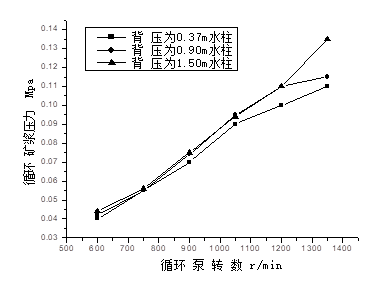
\includegraphics[]{figures/example.png}
    \caption{循环矿浆压力与柱体背压的关系}{Relationship between the pressure of circulating pulp and the back pressure}
    \label{circulating-pulp-and-the-backpressure-relationship} % label 用来在文中索引
\end{figure}

\chapter{浮选柱实验研究}{Experiment Research of Column Flotation}
\section{浮选柱研究现状}{Present Research of Column Flotation}
\begin{algorithm}
    \caption{An algorithm with caption}\label{alg:cap}
    \begin{algorithmic}[1]
        \Require $n \geq 0$
        \Ensure $y = x^n$
        \State $y \gets 1$
        \State $X \gets x$
        \State $N \gets n$
        \While{$N \neq 0$}
        \If{$N$ is even}
            \State $X \gets X \times X$
            \State $N \gets \frac{N}{2}$  \Comment{This is a comment}
        \ElsIf{$N$ is odd}
            \State $y \gets y \times X$
            \State $N \gets N - 1$
        \EndIf
        \EndWhile
    \end{algorithmic}
\end{algorithm}
\chapter{关于参考文献}{About references}

只列出作者直接阅读过或在正文中被引用过的文献资料。引用他人成果,在引文前后必须加双引号,并标明序号,在参考文献中列出。
参考文献中先列出直接引用过的资料,再列出直接阅读过且被参考的资料。参考文献要另起一页,一律放在正文之后,不得放在各章节之后。
根据《中国高校自然科学学报编排规范》的要求书写参考文献,并按顺序编码制,作者只写到第三位,余者写“等”。


几种主要参考文献的格式为:
专(译)著:作者.书名(译者).出版地:出版者,出版年,起止页码\\
连续出版物:作者.文题.刊名.年,卷号(期号):起止页码\\
论 文 集:作者.文题.编者.文集名.出版地:出版者,出版年,起止页码\\
学位论文:作者.文题[博士(或硕士)学位论文].授予单位,授予年~\cite{许家林1999岩层移动与控制的关键层理论及其应用}\\
技术标准:发布单位.技术标准代号.技术标准名称.出版地:出版者,出版日期\\
英文论文~\cite{1978Indexing}


举例如下:
〔例文〕 在出任约翰·霍普金斯大学校长的就职演说中,
吉尔曼阐述了自己的英才主义教育思想:“最慷慨地促进一切有用知识的发展;鼓励研究;
促进青年人的成长,促进那些依靠其能力而献身科学进步的学者的成长”~\cite{贺国庆1998德国和美国大学发达史}。 
吉尔曼按照这一思想,在长达25年的校长任期内,把研究生教育放在首位,并全力以赴地发展科学研究,
取得了堪称辉煌的办学成就。据1926年的调查统计,当时每一千位著名的美国科学家中,就有243人是约翰·霍普金斯大学的毕业生~\cite{陈树清1982美国研究生教育发展的历程及其特点} 。
参考文献(四号、黑体、顶格)


说明:本模板使用此前现有的bst文件,由于网络上(百度学术,谷歌学术等)得到的bib格式可能会有缺失项,导致输出项目并不完全准确。

\chapter{结论}{Conclusion}
本文从自然因素、外部环境和内部结构等方面,详细分析了影响我国煤炭供给和需求的因素,
探索煤炭供需与其影响因素的规律,构建了我国煤炭供需预测预警指标体系,
对我国煤炭供需进行预测预警。
(1) 我国的煤炭供给受许多因素度影响,而且随着时间的推移,出现新的特点。
目前,我国的铁路运输压力又所缓解,但铁路运输还是制约着我国的煤炭供给。
我国煤炭资源区域分异现象与经济区域分异性相悖,由此造成了“西煤东调”和“北煤南运”的运输格局,
这种能源中心与经济中心的差异性,形成了大量的煤炭运输需求以及非常集中的煤炭流量,
但因资金的缺口及体制的原因,铁路运输现在将来一段时期都制约着我国的煤炭供给。


% 正文后部分
\backmatter
% TODO: 参考文献格式.bst和参考文献.bib使用cumt.bst
\bibliographystyle{biblio/cumt}
% \bibliographystyle{biblio/cumt-num}
% \bibliographystyle{biblio/new-cumt-num}
\bibliography{biblio/RefExam}
% 简历
% \begin{resume}

\section*{一、基本情况}


姓名: \zuozhe\quad 性别: 男\quad 民族: 汉\quad 出生年月: 1992-02\quad 籍贯: 江苏扬州

2010-09 --- 2014-07\quad  中国矿业大学环境与测绘学院工学学士;

2014-09 --- 2017-06\quad  中国矿业大学环境与测绘学院工学硕士研究生.

\section*{二、学术成果}

\begin{enumerate}
  \item \zuozhe,土地确权内业处理软件,软件著作权,登记号:2015SR091014
\end{enumerate}


\section*{三、获奖情况}
\begin{enumerate}
  \item 2014-2015年度\quad 一等奖学金
  \item 2015-2016年度\quad 二等奖学金
  \item 2016-2017年度\quad 三等奖学金
\end{enumerate}
\section*{四、研究项目}
\begin{enumerate}
  \item 国家高分重点项目:中科院电子所苏州研究院, 2016, 参与;
  \item 国家自然基金项目:数字摄影测量目标精密定位于精度估计研究,编号:41171343, 参与;
  \item 山东省梁山县农村土地确权登记颁证项目,2014, 主要参与;
\end{enumerate}

\end{resume}

\GuanJianCi{浮选,旋流,分选机理,浮选动力学,矿物分选}
\BingLieTiMing{Analysis and Data Mining about Spatial Data of Sina Weibo Based on Spatial-Spark}
\LunWenYuZhong{中文}
\XueHao{TS14160005}
\PeiYangDanWeiDaiMa{10290}
\PeiYangDanWeiDiZhi{江苏省徐州市}
\XueZhi{四年}
\LunWenTiJiaoRiQi{2022 年 6 月}
\DaBianWeiYuanHuiChengYuan{王永波,杨化超,陈国良,刘志平}
\LunWenZiZhu{无}
\XueWeiShouYuDanWeiMingCheng{}
\XueWeiShouYuDanWeiDaiMa{}
\XueWeiJiBie{}
\LunWenTiMing{}
\PeiYangDanWeiMingCheng{}
\YouBian{}
\XueWeiShouYuNian{}

\makebackcover
\printindex
\clearpage
\end{document}
